

\chapter{Calculus}\label{chapter:calculus}
\begin{figure}[H]
  \centering 
  \begin{tikzpicture}
    \begin{scope}[every node/.style={inner sep=0.5cm}, font=\ttfamily\scriptsize, anchor = east, rounded corners, line width = 0.4mm]
  \node[align=left, fill=sourceBackground, draw=sourceHighlight] (source-program) {\,\$(\textbf{do}$\, x \leftarrow \equote[\return{0}]$\\
  \,\quad \textbf{in} $(\lambda z. \return{z})(x))$};
  \node[align=left, fill=coreBackground, draw=coreHighlight] (core-program) at ($(source-program.east) + (6.4cm, 0cm)$){\textbf{tls}(\textbf{do}$\, x \leftarrow \return{\texttt{Ret}(\texttt{Nat}(0))}$ \\ 
  \quad\quad\textbf{in} $(\lambda z. \return{z})(x)$$)$};

  \node[align=left, fill=effBackground, draw=effHighlight] (normal-form) at ($(core-program.east) + (4cm, 0cm)$) {Ret$($Nat$(0))$\\ };
  \end{scope}

  \begin{scope}[every node/.style={font = \scriptsize}]
    \node[fill=sourceHighlight] (source-lang) at ($(source-program.south) + (0cm, 0cm)$ ) {\textcolor{white}\sourceLang{}};
    \node[fill=coreHighlight] (core-lang) at ($(core-program.south) + (0cm, 0cm)$ ) {\textcolor{white}\coreLang{}};
    \node[fill=effHighlight] (eff-lang) at ($(normal-form.south) + (0cm, 0cm)$ ) {\textcolor{white}\efflang{}};
  \end{scope}

  \begin{scope}[scale=8]
  \node[] (elaboration) at ($(source-program.east) + (0.095cm, -0.004cm)$) {\Huge$\leadsto$};
  \node[] (execution) at ($(core-program.east) + (0.095cm, 0.005cm)$) {\Huge$\rightarrow^{\text{\normalsize{$*$}}}$};
  \end{scope}

  \begin{scope}[every node/.style={font = \sffamily\tiny, anchor = south}]
  \node[] (elaboration-caption) at ($(elaboration) + (0cm, 0.3cm)$) {\textbf{Elaboration}};
  \node[align=center] (execution-caption) at ($(execution) + (0cm, 0.3cm)$) {\textbf{Compile-Time} \\ \textbf{Execution}};
  \end{scope}

  \end{tikzpicture}
  
  \caption{\calculusName{} is first elaborated into \coreLang{}, which is then executed \textbf{at compile-time} to obtain the AST of a run-time \efflang{} program.}%
  \label{fig:elaboration-then-execution}
\end{figure}

This thesis considers the interaction between homogenous, compile-time, two-stage \textbf{metaprogramming} (\Cpageref{section:metaprogramming-technical}), and an \textbf{effect system} with deep handlers and multi-shot continuations (\Cpageref{section:effects-technical}). This chapter describes a calculus, \calculusName{}, for studying said interaction.\ \calculusName{} will have both metaprogramming and effect handlers. To the best of my knowledge, this is the first calculus in which one may write effectful compile-time code that generates effectful run-time code. However, \calculusName{} will not mediate the interaction between metaprogramming and effects: scope extrusion prevention is not a language feature. Rather, the aim will be to extend \calculusName{} with various scope extrusion checks, such that the checks may be evaluated in a comparative fashion. 

Programs written in \calculusName{} cannot be directly executed. Rather, following the style of \citet{xie-2023}, one must first elaborate (or compile) from \calculusName{} (the ``source'' language) to a ``core'' language,\, \coreLang{}.\, Programs written in \coreLang{} may then be executed, to obtain the AST of a run-time \efflang{} program. This process is summarised in \Cref{fig:elaboration-then-execution}. Elaboration is necessary, since it is the point at which dynamic checks may be inserted. 

In this chapter, I will first introduce \sourceLang{} (\Cref{section:source-lang}), then \coreLang{} (\Cref{section:core-lang}). Following this, I will describe the elaboration from \sourceLang{} to \coreLang{} (\Cref{section:elaboration}). Finally, I will discuss the metatheoretic properties of \calculusName{} (\Cref{section:metatheory}). 
% At a high-level, however, the names are suggestive: \sourceLang{} extends \efflang{} with quotation $\equote$ and splicing $\splice$, and \coreLang{} extends \efflang{} with AST constructors. 

\section{The Source Language: \texorpdfstring{\sourceLang{}}{Lambda-Op-Quote-Splice}}\label{section:source-lang}
\begin{figure}
\begin{source-desc}
  {\large \textbf{Syntax}} \\

  $\begin{array}{@{}llll}
    \textbf{Values} & v & ::= & \ldots \\
    \textbf{Expressions} & e & ::= & \ldots \mid \equote \mid \splice
  \end{array}$
\end{source-desc}
\caption{\sourceLang{} syntax. The syntax is broadly the same as \efflang{}, except with the addition of quotes and splices.}
\label{fig:source-syntax}
\end{figure}
\sourceLang{} extends \efflang{} with quotes and splices. Recall that \efflang{} divides terms into two syntactic categories, values $v$ and computations $c$. \sourceLang{} is similar, dividing terms into values $v$ and expressions $e$ (\Cref{fig:source-syntax})

Notice that we cannot quote values: we \textit{must} generate effectful programs. For example, $\equote[1]$ is not valid syntax, instead, one must write $\equote[\return{1}]$. Similarly, $\equote[\return{1}]$ is a computation, not a value, so one must write 
\[\bind{a}{\equote[\return{1}]}{\op{a}}\]
rather than $\op{\, \equote[\return{1}] \,}$. However, in both cases, I will abuse notation for clarity.

\subsection{Type System}
\begin{figure}
  \begin{source-desc}
    $\begin{array}{lllr}
    {\textbf{\large {Effects Row}}}\\\\
    \textbf{Run-Time} & \xi ::= \cdot \mid \xi \cup \{ \textsf{op}_i^{0}\} \\
    \textbf{Compile-Time} & \Delta ::= \cdot \mid \Delta \cup \{ \textsf{op}_i^{-1}\} \\\\
    \end{array}$

\vspace{5mm}
  $\begin{array}{lllr}
    {\textbf{\large {Types}}}\\\\ \vspace{0.4mm}
    \textbf{Level 0} & \text{Values} & T^0 ::= \mathbb{N}^0 & \text{\footnotesize{naturals}} \\ \vspace{0.4mm}
    && \quad\quad\,\, \mid {(\functionType[\xi]{T_1^0}{T_2^{0}})}^{0} & \text{\footnotesize{functions}} \\ \vspace{0.4mm}
    && \quad\quad\,\, \mid {(\continuationType[\xi]{T_1^0}{T_2^{0}})}^{0} & \text{\footnotesize{continuations}} \\\vspace{0.4mm}
    & \text{Computations} & T^0 \, ! \, \xi \\\vspace{0.8mm}
     && \mid T^0 \, ! \,  \Delta;\xi & \\\vspace{0.8mm}
    & \text{Handlers} & (\handlerType{T_1^{0} \, ! \, \xi}{T_2^{0} \, ! \, \xi'})\, !\, \Delta\\ \\ 

    \textbf{Level $-$1} & \text{Values} & T^{-1} ::= \mathbb{N}^{-1} & \text{\footnotesize{naturals}} \\ \vspace{0.4mm}
    && \quad\quad\quad \mid {(\functionType{T_1^{-1}}{T_2^{-1}})}^{-1} & \text{\footnotesize{functions}} \\\vspace{0.4mm}
    && \quad\quad\quad \mid {(\continuationType{T_1^{-1}}{T_2^{-1}})}^{-1} & \text{\footnotesize{continuations}} \\\vspace{0.4mm}
    && \quad\quad\quad \mid {\textsf{Code}({T^{0} \, ! \, \xi})}^{-1} & \text{\footnotesize{run-time code}} \\\vspace{0.8mm}
    & \text{Computations} & T^{-1} \, ! \, \Delta \\\vspace{0.8mm}
    & \text{Handlers} & \handlerType{T_1^{-1} \, ! \, \Delta}{T_2^{-1} \, ! \, \Delta'}
  \end{array}$
  \end{source-desc}
  \caption{\sourceLang{} types. I highlight three important elements: first, types are stratified into two levels, $0$ and $-1$. Second, effects are stratified into two levels, $\xi$ (for run-time effects) and $\Delta$ for compile-time effects. Third, the \textsf{Code} type allows for compile-time programs to manipulate ASTs of run-time code.}
  \label{fig:source-types}
\end{figure}

I will now introduce the \sourceLang{} type system. The \sourceLang{} types are summarised in \Cref{fig:source-types}. I highlight three important details: types are stratified into two levels ($-1$ for compile-time and $0$ for run-time), effect rows are similarly stratified, and run-time code is made available at compile-time via a \textsf{Code} type.

First, \textbf{types are stratified into two levels, $T^0$ (run-time), and $T^{-1}$ (compile-time).}

  To motivate this stratification, consider the following question: what is the type of the number $3$ in \sourceLang{}? Perhaps surprisingly, the answer is not $\mathbb{N}$. Since we are working with a two-stage system, we must be careful to disambiguate between run-time naturals and compile-time naturals, since these are not interchangeable. For example, the following program should \textbf{not} be well-typed, since $3$ is a compile-time natural, whereas $x$ is a run-time natural. 
  \[\lambda x: \mathbb{N}. \, \$(3 + x)\]
  However, removing the splice makes the program well-typed
  \[\lambda x: \mathbb{N}. \, 3 + x\]
  Following \citet{xie-2023}, I introduce integer levels to enforce separation between compile-time and run-time naturals. While the precise notion of level is slightly more involved (see below), for my purposes, it is sufficient to think of level $0$ as run-time (so $\mathbb{N}^0$ is a run-time natural), and $-1$ as compile-time. The ill-typed example becomes
  \[\lambda x: \mathbb{N}^0. \, \$(\textcolor{comment}{(\textcolor{black}{3}:\mathbb{N}^{-1})} + \textcolor{comment}{(\textcolor{black}{x}:\mathbb{N}^{0})})\]
  and the well-typed example 
  \[\lambda x: \mathbb{N}^0. \, \textcolor{comment}{(\textcolor{black}{3}:\mathbb{N}^{0})} + \textcolor{comment}{(\textcolor{black}{x}:\mathbb{N}^{0})}\]
  More precisely, levels are defined as follows:

  \begin{definition}[Level]{sourceHighlight}
    The level of an expression $e$ is calculated by subtracting the number of surrounding splices from the number of surrounding quotations.
  \end{definition}

  The definition of level generalises to multi-stage languages, where negative levels ($-1, -2, \ldots$) represent compile-time and non-negative levels ($0, 1, \ldots$) represent run-time. In a multi-staged language, separation is even more granular: for example, level $1$ and level $0$ run-time naturals are disambiguated. However, since I only deal with two stages, it is sufficient to consider only levels $0$ and $-1$. The definition, and the examples above, further imply that the ``default'' level, in the absence of quotes and splices, is level $0$. Intuitively, in the absence of quotes and splices, the programmer is ignoring metaprogramming facilities, and constructing a run-time program. 


  Notice that the opening question was slightly devious\footnote{sorry}! We cannot assign a type to \textit{program fragments}, like $3$, since without knowledge of the wider context, we cannot know which level we are at: in the ill-typed example, $3$ occurs under a splice, but no quotes, so it has type $\mathbb{N}^{-1}$, and in the well-typed example, it has type $\mathbb{N}^0$. Unless otherwise stated, I will always assume program fragments occur at level $0$.

  Second, \textbf{effect rows are stratified into $\xi$ (run-time) and $\Delta$ (compile-time).}\\
  In the following example, we print $1$ at compile-time, and $2$ at run-time. Further, we read an integer at run-time.
\[\splice[{(\textbf{\texttt{print}}(1); \equote[\textbf{\texttt{print}}(2); \textbf{\texttt{readInt}}()])}]\]
Hence, $\Delta = \{ \textbf{\texttt{print}} \}$ and $\xi = \{ \textbf{\texttt{print}}, \textbf{\texttt{readInt}} \}$. We may now disambiguate between different computation types:
\begin{enumerate}[leftmargin=5.8\parindent]
  \item[$T^0 \quad\quad\,\,$] Compile-time value, run-time value (value types) \\
  \textit{Example}: The type of $x$ in $\lambda x. \return{x}$
  \item[$T^0 \, ! \, \xi \quad\;$] Compile-time value, run-time computation  \\
  \textit{Example}: The type of $x$ in $\splice[(\bind{x}{\equote[\return{1}]}{\return{x}})]$
  \item[$T^0 \, ! \, \Delta \quad$] Compile-time computation, run-time value \\
  \textit{Example}: $\lambda x. \return{x}$ 
  \item[$T^0 \, ! \, \Delta; \xi$] Compile and run-time computation \\
  \textit{Example}: $\splice[(\bind{x}{\equote[\return{1}]}{\return{x}})]$
\end{enumerate}
% As a result of the type system, we never encounter $T^0 \, ! \, \Delta$ (compile-time computations that are run-time values).

Third, \textbf{there is an level $-1$ \textsf{Code} type, representing run-time ASTs.}\\ 
  By stratifying types, we have ensured that run-time (resp.\ compile-time) terms only interact with run-time (compile-time) terms. However, to enable meta-programming, run-time terms \textit{should be available} at compile-time as ASTs. This is exactly the role of the \textsf{Code} type, thus allowing level $-1$ programs to manipulate ASTs of level $0$ terms.
% Note that if we had a multi-level system, then there would be a \texttt{Code} type at level $0$, representing the ASTs of level $1$ terms. The asymmetry arises from the restriction to two levels. 

Putting it all together, we can now interpret complex \sourceLang{} types, like 
\begin{center}
\begin{tikzpicture}

  \begin{scope}[local bounding box=group 1]
  \node[text width=\linewidth, align = center] (example) at (0, 0) {$(\functionType[]{{\textsf{Code}(\mathbb{N}^0 ! \{ \texttt{print} \})}^{-1}}{\textsf{Code}(\mathbb{N}^0 \, ! \, \{ \texttt{print}, \texttt{readInt} \})^{-1}})^{-1}$};
  '\end{scope}

  \node[align=center, font=\footnotesize](effects) at (-1.1cm,0.3cm){$\{ \texttt{get} \}$};

  \begin{scope}[on background layer, font=\scriptsize\bfseries, text=comment, align=left]
    \draw[draw=comment, line width = 0.3mm] ($(example.north east) + (-3.1cm, 0.6cm)$) circle[radius=1.4mm] node (annote-1) {\tiny{1}};
    \node[anchor = east, align=right] (annote-1-text) at ($(annote-1.west) + (0.1cm, -0.15cm)$) {Compile-time \\function} ;
    \draw[draw=comment, line width =0.3mm] ($(example.north east) + (-2.6cm, 0cm)$) |- (annote-1.east);

    \draw[draw=comment, line width = 0.3mm] ($(effects.north) + (-0.5cm, 0.4cm)$) circle[radius=1.4mm] node (annote-2) {\tiny{2}};
    \node[anchor = east, align=right] (annote-2-text) at ($(annote-2.west) + (0.1cm, -0.15cm)$) {Compile-time \\effects} ;
    \draw[draw=comment, line width =0.3mm] (effects.north) |- (annote-2.east);

    \draw[draw=comment, line width = 0.3mm] ($(example.south west) + (3.4cm, -0.4cm)$) circle[radius=1.4mm] node (annote-3) {\tiny{3}};
    \node[anchor = north west, align=left] (annote-3-text) at ($(annote-3.east) + (-0.1cm, 0.27cm)$) {Input: AST of a run-time \\ computation of type $\mathbb{N} \, ! \, \{\texttt{print}\}$} ;
    \draw[draw=comment, line width =0.3mm] ($(example.south west) + (2.9cm, 0cm)$) |- (annote-3.west);

    \draw[draw=comment, line width = 0.3mm] ($(example.south east) + (-7.5cm, -0.4cm)$) circle[radius=1.4mm] node (annote-4) {\tiny{4}};
    \node[anchor = north west, align=left] (annote-4-text) at ($(annote-4.east) + (-0.1cm, 0.27cm)$) {Output: AST of a run-time \\ computation of type $\mathbb{N} \, ! \, \{\texttt{print},\texttt{readInt}\}$} ;
    \draw[draw=comment, line width =0.3mm]  ($(example.south east) + (-8cm, 0cm)$) |- (annote-4.west);
  \end{scope}

\end{tikzpicture}


\end{center}
% Reading from the outside-in:
% \begin{enumerate}
%   \item This is a level $-1$, or compile-time function
%   \item The function has (suspended) compile-time effect \texttt{get} 
%   \item The function expects an AST of some run-time computation with type with type $\mathbb{N} \, ! \, \{\texttt{print}\}$
%   \item The function returns an AST of some run-time computation with type $\mathbb{N} \, ! \, \{\texttt{print},\texttt{readInt}\}$
% \end{enumerate}
\subsubsection{Typing Judgement}
Having described the types, I now present the type system. The typing rules are collated in \Cref{fig:source-cq-typing-rules,fig:source-s-typing-rules}. I will first explain the typing judgement, then highlight some key rules. 

The shape of the typing judgement is mostly familiar, though, as in \citet{xie-2023}, I add level information and compiler modes. Level information will turn out to be redundant, but we will revisit this later.
\[\Gamma \vdash^{\text{Level}}_{\text{Mode}} e: T\]
% I shall explain these in turn. 

\textbf{Level}. Recall that, when describing the \efflang{} types, I argued that one cannot type a program fragment, like $3$, directly. One must also know the \textit{level} ($0$ or $-1$), which is accordingly attached to the typing judgement.


\newcommand{\compilemode}{\textbf{\textsf{\textcolor{compile}{c}}}}
\newcommand{\splicemode}{\textbf{\textsf{\textcolor{splice}{s}}}}
\newcommand{\quotemode}{\textbf{\textsf{\textcolor{quote}{q}}}}
\textbf{Mode}. For the purposes of elaboration, it can be useful to classify code into three categories:

\begin{enumerate}
  \item[\compilemode] Code that is \textcolor{compile}{\textbf{ambient}} and \textcolor{compile}{\textbf{inert}}.\\
  \textit{No surrounding quotes or splices}
  \item[\splicemode] Code that \textcolor{splice}{\textbf{manipulates ASTs}} at compile-time. \\
  \textit{Last surrounding annotation is a splice}
  \item[\quotemode] Code that \textcolor{quote}{\textbf{builds ASTs}} to be manipulated at compile time. \\
  \textit{Last surrounding annotation is a quote}
\end{enumerate}

To illustrate the purpose of the modes, consider the following meta-program, which evaluates to the AST of $\lambda x. 1+2+3$. This program adopts the shorthand of \Cref{subsection:effect-handler-calculus}, where \texttt{\textbf{return}}s are implicitly inserted (for example, $\equote[1]$ should really be $\equote[\return{1}]$), and we elide the order of operation ($1+2$ should really be written out using \textbf{\texttt{do}}). The emphasis is on the three modes:

\begin{center}
  \begin{tikzpicture}
  \node (example) {$\lambda x. \, \splice[(\bind{f}{(\lambda y. \equote[{\splice[(y)] + 2}])}{\bind{a}{\equote[1]}{f a}})] +3$};
  \draw[fill = compile, draw=compile, anchor = north west] ($(example.south west) + (0.05cm, 0.06cm)$) rectangle ($(example.south west) + (0.7cm, -0cm)$);
  \node[anchor=north] at ($(example.south west) + (0.375cm, -0.1cm)$) {\compilemode{}};
  \draw[fill = splice, draw=splice, anchor = north west] ($(example.south west) + (1.2cm, 0.06cm)$) rectangle ($(example.south west) + (3.3cm, -0cm)$);
  \node[anchor=north] at ($(example.south west) + (2.25cm, -0.1cm)$) {\splicemode{}};
  \draw[fill = splice, draw=splice, anchor = north west] ($(example.south west) + (4.08cm, 0.06cm)$) rectangle ($(example.south west) + (4.28cm, -0cm)$);
  \node[anchor=north] at ($(example.south west) + (4.18cm, -0.1cm)$) {\splicemode{}};
  \draw[fill = quote, draw=quote, anchor = north west] ($(example.south west) + (4.58cm, 0.06cm)$) rectangle ($(example.south west) + (5.15cm, -0cm)$);
  \node[anchor=north] at ($(example.south west) + (4.8655cm, -0.1cm)$) {\quotemode{}};
  \draw[fill = splice, draw=splice, anchor = north west] ($(example.south west) + (5.8cm, 0.06cm)$) rectangle ($(example.south west) + (7.65cm, -0cm)$);
  \node[anchor=north] at ($(example.south west) + (6.7cm, -0.1cm)$) {\splicemode{}};
  \draw[fill = quote, draw=quote, anchor = north west] ($(example.south west) + (8.07cm, 0.06cm)$) rectangle ($(example.south west) + (8.27cm, -0cm)$);
  \node[anchor=north] at ($(example.south west) + (8.17cm, -0.1cm)$) {\quotemode{}};
  \draw[fill = splice, draw=splice, anchor = north west] ($(example.south west) + (8.75cm, 0.06cm)$) rectangle ($(example.south west) + (9.75cm, -0cm)$);
  \node[anchor=north] at ($(example.south west) + (9.25cm, -0.1cm)$) {\splicemode{}};
  \draw[fill = compile, draw=compile, anchor = north west] ($(example.south west) + (9.95cm, 0.06cm)$) rectangle ($(example.south west) + (10.65cm, -0cm)$);
  \node[anchor=north] at ($(example.south west) + (10.35cm, -0.1cm)$) {\compilemode{}};
  \end{tikzpicture}
  \end{center}

\begin{enumerate}
  \item[\compilemode] Identifies AST nodes that are \textcolor{compile}{\textbf{ambient}} (within which computation may take place) and \textcolor{compile}{\textbf{inert}} (cannot themselves be manipulated at compile-time). 
  
\begin{center}
  \begin{tikzpicture}
  \node (example) {$\lambda x. \, \splice[(\bind{f}{(\lambda y. \equote[{\splice[(y)] + 2}])}{\bind{a}{\equote[1]}{f a}})] +3$};
  \draw[fill = compile, draw=compile, anchor = north west] ($(example.south west) + (0.05cm, 0.06cm)$) rectangle ($(example.south west) + (0.7cm, -0cm)$);
  \draw[fill = compile, draw=compile, anchor = north west] ($(example.south west) + (9.95cm, 0.06cm)$) rectangle ($(example.south west) + (10.65cm, -0cm)$);
  \end{tikzpicture}
  \end{center}
  \item[\splicemode] Identifies code that can be executed at compile-time to \textcolor{splice}{\textbf{manipulate ASTs}}. Will be fully reduced at compile-time, and will not appear at run-time. 
  \begin{center}
  \begin{tikzpicture}
  \node (example) {$\lambda x. \, \splice[(\bind{f}{(\lambda y. \equote[{\splice[(y)] + 2}])}{\bind{a}{\equote[1]}{f a}})] +3$};
  \draw[fill = splice, draw=splice, anchor = north west] ($(example.south west) + (1.2cm, 0.06cm)$) rectangle ($(example.south west) + (3.3cm, -0cm)$);
  \draw[fill = splice, draw=splice, anchor = north west] ($(example.south west) + (4.08cm, 0.06cm)$) rectangle ($(example.south west) + (4.28cm, -0cm)$);
  \draw[fill = splice, draw=splice, anchor = north west] ($(example.south west) + (8.75cm, 0.06cm)$) rectangle ($(example.south west) + (9.75cm, -0cm)$);
  \end{tikzpicture}
  \end{center}

  \item[\quotemode] Identifies code that \textcolor{quote}{\textbf{builds ASTs}} (like \compilemode-mode) that can be manipulated at compile-time (unlike \compilemode-mode), to create run-time programs. 
\begin{center}
  \begin{tikzpicture}
  \node (example) {$\lambda x. \, \splice[(\bind{f}{(\lambda y. \equote[{\splice[(y)] + 2}])}{\bind{a}{\equote[1]}{f a}})] +3$};
  \draw[fill = quote, draw=quote, anchor = north west] ($(example.south west) + (4.58cm, 0.06cm)$) rectangle ($(example.south west) + (5.15cm, -0cm)$);
  \draw[fill = quote, draw=quote, anchor = north west] ($(example.south west) + (8.07cm, 0.06cm)$) rectangle ($(example.south west) + (8.27cm, -0cm)$);
  \end{tikzpicture}
  \end{center}
  \end{enumerate}

We may also describe how \textit{transitions} between modes occur:
\begin{enumerate}
  \item Top-level splices ($\splice$) transition from \compilemode{} (outside the splice) to \splicemode{} (within).
  \item Quotes ($\equote[e]$) transition from \splicemode{} (outside the quote) to \quotemode{} (within).
  \item Splices ($\splice$) transition from \quotemode{} (outside the splice) to \splicemode{} (within).
\end{enumerate}
Transitions between modes are illustrated in \Cref{fig:compiler-mode-transitions}.

\begin{figure}
  \centering
\begin{tikzpicture}[->,>=stealth']
  \node (c) {\Large\textbf{\textsf{\textcolor{compile}{c}}}}; 
  \node (s) at ($(c.east) + (2cm, 0cm)$) {\Large\textbf{\textsf{\textcolor{splice}{s}}}};
  \node (q) at ($(s.south) + (0cm, 2cm)$) {\Large\textbf{\textsf{\textcolor{quote}{q}}}};
  
  \draw (c) to node[anchor=north, font=\footnotesize, align=center]{$\splice$ \\ (top-level)} (s);

  \draw (s.north east) to[out=40, in=-40] node[anchor=west, font=\footnotesize]{$\equote$} (q.south east);
  \draw (q.south west) to[out=-140, in=140] node[anchor=east, font=\footnotesize]{$\splice$} (s.north west);

\end{tikzpicture}
\caption{Transitions between modes \compilemode{}, \splicemode{}, and \quotemode{}. Top-level splices transition from \compilemode{} to \splicemode{}, quotes transition from \splicemode{} to \quotemode{}, and splices (under quotes) transition from \quotemode{} to \splicemode{}.}%
\label{fig:compiler-mode-transitions}
\end{figure}

Since \sourceLang{} has only two levels, and my type system will ban nested splices and quotations ($\splice[\splice]$ and $\equote[\equote]$ are not valid program fragments), the compiler mode will uniquely identify the level (\compilemode{} and \quotemode{} imply level $0$, and \splicemode{} level $-1$). I thus drop the level from my typing judgement, leaving it implicit.

\newcommand{\cqtypejudge}[3][\Gamma]{{#1} \vdash_{\compilemode \mid \quotemode} {#2} : {#3}}
\newcommand{\ctypejudge}[3][\Gamma]{{#1} \vdash_{\compilemode} {#2} : {#3}}
\newcommand{\qtypejudge}[3][\Gamma]{{#1} \vdash_{\quotemode} {#2} : {#3}}
\newcommand{\stypejudge}[3][\Gamma]{{#1} \vdash_{\splicemode} {#2} : {#3}}

\newcommand{\runtimecomptype}[2]{{#1}^0 \, ! \, {#2}}
\newcommand{\compiletimetype}[1]{{#1}^{-1}}
\newcommand{\compiletimecomptype}[2]{{#1}^{-1} ! {#2}}

Further, the typing judgements for \compilemode{} and \quotemode{} will be identical in almost all cases. To avoid repetition, I introduce the following notation
\[\cqtypejudge{e}{T}\]
Where, for example, the typing rule 
\[\inferrule{\cqtypejudge[\Gamma_1]{e_1}{T_1} \\ \cdots \\ \cqtypejudge[\Gamma_n]{e_n}{T_n} }{\cqtypejudge{e}{T}}\]
stands for two typing rules, one in \compilemode{}-mode and one in \quotemode{}-mode.
\begin{center}
\begin{minipage}[t]{0.3\textwidth}
  \centering 
  $\inferrule{\ctypejudge[\Gamma_1]{e_1}{T_1} \\\\ \cdots \\\\ \ctypejudge[\Gamma_n]{e_n}{T_n} }{\ctypejudge{e}{T}}$
\end{minipage}%
\begin{minipage}[t]{0.3\textwidth}
  \centering
  $\inferrule{\qtypejudge[\Gamma_1]{e_1}{T_1} \\\\ \cdots \\\\ \qtypejudge[\Gamma_n]{e_n}{T_n} }{\qtypejudge{e}{T}}$
\end{minipage}
\end{center}

The \compilemode{} and \quotemode{}-mode typing rules are summarised in \Cref{fig:source-cq-typing-rules}. The \splicemode{}-mode typing rules are summarised in \Cref{fig:source-s-typing-rules}. In all modes, rules are extremely similar to the \efflang{} typing rules (\Cref{fig:efflang-type-system}, \Cpageref{fig:efflang-type-system}). I focus on three important rules: \textsc{\splicemode{}-Quote}, \textsc{\quotemode{}-Splice}, and \textsc{\compilemode{}-Splice}. 


\begin{figure}
\begin{source-desc}
  {\large\textbf{\compilemode{} and \quotemode{} Typing Rules}}

  \begin{center}
  \begin{minipage}[t]{0.3\textwidth}
    \centering
    $\inferrule[(Nat)]{ \\ }{\cqtypejudge{m}{\runtimecomptype{\mathbb{N}}{\Delta}}}$
  \end{minipage}%
  \begin{minipage}[t]{0.3\textwidth}
    \centering
    $\inferrule[(Var)]{\Gamma(x) = T^0}{\cqtypejudge{x}{\runtimecomptype{T}{\Delta}}}$
  \end{minipage}%
  \begin{minipage}[t]{0.4\textwidth}
    \centering
$\inferrule[(Lambda)]{\cqtypejudge[\Gamma, x: T_1^0]{e}{\runtimecomptype{T_2}{\Delta;\xi}}}{\cqtypejudge{\lambda x.e}{\runtimecomptype{(\functionType[\xi]{T_1^0}{T_2^0})}{\Delta}}}$
\end{minipage}

\vspace{5mm}

\begin{minipage}[t]{0.5\textwidth}
\centering
$\inferrule[(App)]{\cqtypejudge[\Gamma]{v_1}{\runtimecomptype{(\functionType[\xi]{T_1^0}{T_2^0})}{\Delta}} \\ \cqtypejudge[\Gamma]{v_2}{\runtimecomptype{T_1}{\Delta}}}{\cqtypejudge{v_1 v_2}{\runtimecomptype{T_2}{\Delta;\xi}}}$
\end{minipage}%
\begin{minipage}[t]{0.5\textwidth}
  \centering
  $\inferrule[(Continue)]{\cqtypejudge[\Gamma]{v_1}{\runtimecomptype{(\continuationType[\xi]{T_1^0}{T_2^0})}{\Delta}} \\ \cqtypejudge[\Gamma]{v_2}{\runtimecomptype{T_1}{\Delta}}}{\cqtypejudge{\continue{v_1}{v_2}}{\runtimecomptype{T_2}{\Delta;\xi}}}$
  \end{minipage}

  \vspace{5mm}

  \begin{minipage}[t]{0.45\textwidth}
    \centering
    $\inferrule[(Return)]{  \\\\ \cqtypejudge[\Gamma]{v}{\runtimecomptype{T}{\Delta}}}{\cqtypejudge{\return{v}}{\runtimecomptype{T}{\Delta;\xi}}}$
  \end{minipage}%
  \begin{minipage}[t]{0.45\textwidth}
    \centering
    $\inferrule[(Do)]{\cqtypejudge[\Gamma]{e_1}{\runtimecomptype{T_1}{\Delta;\xi}} \\ \cqtypejudge[\Gamma, x:T_1^0]{e_2}{\runtimecomptype{T_2}{\Delta;\xi}}}{\cqtypejudge{\bind{x}{e_1}{e_2}}{\runtimecomptype{T_2}{\Delta;\xi}}}$
  \end{minipage}

\vspace{5mm}

\begin{minipage}[t]{0.5\textwidth}
  \centering
  $\inferrule[(Op)]{  \\\\ \cqtypejudge[\Gamma]{v}{\runtimecomptype{T_1}{\Delta}} \\ \texttt{op}: T_1^0 \to T_2^0 \in \Sigma \\ \texttt{op} \in \xi}{\cqtypejudge{\op{v}}{\runtimecomptype{T_2}{\Delta;\xi}}}$
\end{minipage}%
\begin{minipage}[t]{0.5\textwidth}
  \centering
  $\inferrule[(Handle)]{\cqtypejudge[\Gamma]{e}{\runtimecomptype{T_1}{\Delta;\xi}} \\ \cqtypejudge{h}{(\handlerType{\runtimecomptype{T_1}{\xi}}{\runtimecomptype{T_2}{\xi'}})\,!\,\Delta} \\ \forall \texttt{op} \in \Delta \setminus \Delta' \, . \, \texttt{op} \in \textsf{dom}(h)}{\cqtypejudge{\handleWith{e}{h}}{\runtimecomptype{T_2}{\Delta;\xi'}}}$
\end{minipage}

\vspace{5mm}

\begin{minipage}[t]{\textwidth}
  \centering
$\inferrule[(Ret-Handler)]{\cqtypejudge[\Gamma, x: T_1^0]{e}{\runtimecomptype{T_2}{\Delta;\xi'}}}{\cqtypejudge{\returnHandler{x}{e}}{(\handlerType{\runtimecomptype{T_1}{\xi}}{\runtimecomptype{T_2}{\xi'}})\,!\,\Delta}}$
\end{minipage}

\vspace{5mm}

\begin{minipage}[t]{1\linewidth}
  \centering
$\inferrule[(Op-Handler)]{\texttt{op}: A^0 \to B^0 \in \Sigma 
\\\\ \cqtypejudge{h}{(\handlerType{\runtimecomptype{T_1}{\xi}}{\runtimecomptype{T_2}{\xi'}})\,!\,\Delta}
\\\\ \cqtypejudge[\Gamma, x: A^0, k: {(\continuationType[\xi']{B^0}{T_2^0})^0} ]{e}{\runtimecomptype{T_2}{\Delta;\xi'}} \\ \xi\ \subseteq \xi \setminus \{ \texttt{op} \} \\ \opHandler{x'}{k'}{e'} \notin h} {\cqtypejudge{h;\opHandler{x}{k}{e}}{(\handlerType{\runtimecomptype{T_1}{\xi}}{\runtimecomptype{T_2}{\xi'}})\,!\,\Delta}}$
\end{minipage}

\vspace{5mm}

\begin{minipage}[t]{0.5\textwidth}
  \centering
  $\inferrule[(\compilemode{}-Splice)]{\stypejudge[\Gamma]{e}{\textsf{Code}(T^0 \, ! \, \xi)^{-1} \, ! \, \Delta}}{\ctypejudge{\splice}{\runtimecomptype{T}{\Delta ; \xi}}}$
\end{minipage}%
\begin{minipage}[t]{0.5\textwidth}
  \centering
  $\inferrule[(\quotemode{}-Splice)]{\stypejudge[\Gamma]{e}{\textsf{Code}(T^0 \, ! \, \xi)^{-1} \, ! \, \Delta}}{\qtypejudge{\splice}{\runtimecomptype{T}{\Delta ; \xi}}}$
\end{minipage}

\end{center}
\end{source-desc}
\caption{The \compilemode{}-mode and \quotemode{}-mode typing rules for \sourceLang{}. The rules are nearly identical to the \efflang{} typing rules, with the exception of level annotations on types. Two additional rules, \textsc{(\compilemode{}-Splice)} (top-level splice) and \textsc{(\quotemode{}-Splice)} formalise the transition to \splicemode{}-mode.}%
\label{fig:source-cq-typing-rules}
\end{figure}

\begin{figure}
  \begin{source-desc}
    {\large\textbf{\splicemode{} Typing Rules}}
    \begin{center} 
    \begin{minipage}[t]{0.2\textwidth}
      \centering
      $\inferrule[(\splicemode{}-Nat)]
      { \\ }
      {\stypejudge{m}{\compiletimetype{\mathbb{N}}}}$
      \end{minipage}%
  \begin{minipage}[t]{0.2\textwidth}
    \centering
  $\inferrule[(\splicemode{}-Var)]
  {\Gamma(x) = \compiletimetype{T}}
  {\stypejudge{x}{\compiletimetype{T}}}$
  \end{minipage}

  \vspace{5mm}

  \begin{minipage}[t]{0.5\textwidth}
    \centering
  $\inferrule[(\splicemode{}-Function)]
  {\stypejudge[\Gamma, x:\compiletimetype{T_1}]{e}{\effectType{\compiletimetype{T_2}}}}
  {\stypejudge{\function{x}{e}}{\compiletimetype{(\functionType{\compiletimetype{T_1}}{\compiletimetype{T_2}})}}}$
  \end{minipage}%
  \begin{minipage}[t]{0.5\textwidth}
  \centering
$\inferrule[(\splicemode{}-Continuation)]
  {\stypejudge[\Gamma, x:\compiletimetype{T_1}]{e}{\effectType{\compiletimetype{T_2}}}}
  {\stypejudge{\continuation{x}{e}}{\compiletimetype{(\continuationType{\compiletimetype{T_1}}{\compiletimetype{T_2}})}}}$
\end{minipage}
  
  \vspace{5mm}
  
  \begin{minipage}[t]{0.5\textwidth}
    \centering
  $\inferrule[(\splicemode{}-App)]
    {\stypejudge{v_1}{\compiletimetype{(\functionType{\compiletimetype{T_1}}{\compiletimetype{T_2}})}} \\ \stypejudge{v_2}{\compiletimetype{T_1}}}
    {\stypejudge{v_1 \, v_2}{\effectType{\compiletimetype{T_2}}}}$
  \end{minipage}%
  \begin{minipage}[t]{0.5\textwidth}
    \centering
  $\inferrule[(\splicemode{}-Continue)]
    {\stypejudge{v_1}{\compiletimetype{(\continuationType{\compiletimetype{T_1}}{\compiletimetype{T_2}})}} \\ \stypejudge{v_2}{\compiletimetype{T_1}}}
    {\stypejudge{\continue{v_1}{v_2}}{\effectType{\compiletimetype{T_2}}}}$
  \end{minipage}

  \vspace{5mm}

  \begin{minipage}[t]{0.45\textwidth}
    \centering
  $\inferrule[(\splicemode{}-Return)]
    {  \\\\ \stypejudge{v}{\compiletimetype{T}}}
    {\stypejudge{\return{v}}{\effectType{\compiletimetype{T}}}}$
  \end{minipage}%
  \begin{minipage}[t]{0.45\textwidth}
    \centering
  $\inferrule[(\splicemode{}-Do)]
    {\stypejudge{e_1}{\effectType{\compiletimetype{T_1}}} \\ \stypejudge[\Gamma, x: T_1]{e_2}{\effectType{\compiletimetype{T_2}}}}
    {\stypejudge{\bind{x}{e_1}{e_2}}{\effectType{\compiletimetype{T_2}}}}$
  \end{minipage}
  
  \vspace{5mm}
  % \begin{minipage}[t]{0.5\textwidth}
  %   \centering
  % $\inferrule[(Do)]
  %   {\stypejudge{c_1}{\effectType{T_1}} \\ \stypejudge[, x: T_1]{c_2}{\effectType{T_2}}}
  %   {\stypejudge{\bind{x}{c_1}{c_2}}{\effectType{T_2}}}$
  % \end{minipage}%
  \begin{minipage}[t]{0.5\textwidth}
    \centering
  $\inferrule[(\splicemode{}-Op)]
    {  \\\\ \stypejudge{v}{\compiletimetype{T_1}} \\ \texttt{op}: \compiletimetype{T_1} \rightarrow \compiletimetype{T_2} \in \Sigma \\ \texttt{op} \in \Delta}
    {\stypejudge{\op{v}}{\effectType{\compiletimetype{T_2}}}}$
  \end{minipage}%
  \begin{minipage}[t]{0.5\textwidth}
    \centering
  $\inferrule[(\splicemode{}-Handle)]
    {\stypejudge{e}{\effectType{\compiletimetype{T_1}}} \\ \stypejudge{h}{\compiletimetype{(\handlerType{\effectType{\compiletimetype{T_1}}}{\effectType[\Delta']{\compiletimetype{T_2}}})}} \\ \forall \textsf{op} \in \Delta \setminus \Delta'. \, \textsf{op} \in \textsf{dom}(h)}
    {\stypejudge{\handleWith{e}{h}}{\effectType[\Delta']{\compiletimetype{T_2}}}}$
  \end{minipage}\\

  \vspace{5mm}

  \begin{minipage}[t]{\textwidth}
    \centering
  $\inferrule[(\splicemode{}-Ret-Handler)]
    {\stypejudge[\Gamma, x:\compiletimetype{T_1}]{e}{\effectType[\Delta']{\compiletimetype{T_2}}}}
    {\stypejudge{\returnHandler{x}{e}}{\compiletimetype{(\handlerType{\effectType{\compiletimetype{T_1}}}{\effectType[\Delta']{\compiletimetype{T_2}}})}}}$
  \end{minipage}
  
  \vspace{5mm}
  % \[\inferrule [(Lam)]
  % {\stypejudge[, x:T_1]{t}{\sEffect{T_2}}}
  % {\stypejudge{\function{x}{t}}{\sFunctionType{T_1}{T_2}}}\]
  
  % \[\inferrule[(App)]
  % {\stypejudge{n_1}{\sFunctionType{T_1}{T_2}} \\
  \begin{minipage}[t]{1\linewidth}
    \centering
  $\inferrule[(\splicemode{}-Op-Handler)]
    { \texttt{op}: \compiletimetype{A} \to \compiletimetype{B} \in \Sigma \\\\ 
      \stypejudge{h}{\compiletimetype{(\handlerType{\effectType{\compiletimetype{T_1}}}{\effectType[\Delta']{\compiletimetype{T_2}}})}}\\
      \stypejudge[\Gamma, x:\compiletimetype{A}, k:{\compiletimetype{(\continuationType[\Delta']{\compiletimetype{B}}{\compiletimetype{T_2}})}} ]{e}{\effectType[\Delta']{\compiletimetype{T_2}}}\\
      \Delta' \subseteq \Delta \setminus \{ \texttt{op} \} \\
             \opHandler{x'}{k'}{e'} \notin h}
    {\stypejudge{h ; \opHandler{x}{k}{e}}{\compiletimetype{(\handlerType{\effectType{\compiletimetype{T_1}}}{\effectType[\Delta']{\compiletimetype{T_2}}})}}}$
  \end{minipage}

  \vspace{5mm}

  \begin{minipage}[t]{\linewidth}
    \centering
    $\inferrule[(\splicemode{}-Quote)]{\qtypejudge{e}{\runtimecomptype{T}{\Delta ; \xi}}}{\stypejudge{\equote}{\effectType{\compiletimetype{\textsf{Code}(\runtimecomptype{T}{\xi})}}}}$
  \end{minipage}

\end{center}
  \end{source-desc}
\caption{The \splicemode{}-mode typing rules for \sourceLang{}. The rules are exactly identical to the \efflang{} typing rules, with the exception of level annotations on types, and the additional \textsc{(Quote)} rule, which makes level $0$ code available at compile-time. }%
\label{fig:source-s-typing-rules}
\end{figure}

Recall that the \textsf{Code} type makes available at compile-time a representation of ASTs of level $0$ programs. Recall further that $\equote$ is the mechanism for \textit{creating} ASTs (elements of type \textsf{Code}) from run-time programs. This intuition is captured by the \textsc{\splicemode{}-Quote} rule, where, to verify that $\equote$ is a valid AST of type \textsf{Code}, we verify that $e$ is a run-time program of the corresponding type.
\[\inferrule[(\splicemode{}-Quote)]{\qtypejudge{e}{\runtimecomptype{T}{\Delta ; \xi}}}{\stypejudge{\equote}{\effectType{\compiletimetype{\textsf{Code}(\runtimecomptype{T}{\xi})}}}}\]

The dual to $\equote$ is $\splice$, which \textit{eliminates} compile-time ASTs by transforming them (back) into run-time code. This intuition is captured by the \textsc{\quotemode{}-Splice} and \textsc{\compilemode{}-Splice} rules, where, to verify that $\splice$ is a valid run-time program, we check that $e$ is a valid compile-time AST of the corresponding type. 

\begin{center}
\begin{minipage}[t]{0.5\textwidth}
  \centering
  $\inferrule[(\compilemode{}-Splice)]{\stypejudge[\Gamma]{e}{\textsf{Code}(T^0 \, ! \, \xi)^{-1} \, ! \, \Delta}}{\ctypejudge{\splice}{\runtimecomptype{T}{\Delta ; \xi}}}$
\end{minipage}%
\begin{minipage}[t]{0.5\textwidth}
  \centering
  $\inferrule[(\quotemode{}-Splice)]{\stypejudge[\Gamma]{e}{\textsf{Code}(T^0 \, ! \, \xi)^{-1} \, ! \, \Delta}}{\qtypejudge{\splice}{\runtimecomptype{T}{\Delta ; \xi}}}$
\end{minipage}
\end{center}

% Further, while the rules are syntactically identical, morally, they ought to be kept separate: \textsc{\compilemode{}-Splice} is the typing rule for top-level splices: the mechanism that turns compile-time ASTs into run-time programs, and then additionally \textit{inserts} them into an \textit{ambient} and \textit{inert} expression. \textsc{\quotemode{}-Splice} is the typing rule for non-top-level splices. While these splices similarly turn compile-time ASTs into run-time programs, the resulting run-time program could be used in a myriad of ways -- used to build larger programs, or discarded entirely. 

Note that since there are no \textsc{\quotemode-Quote} or \textsc{\splicemode-Splice} rules, the type system bans nested splices and quotations, and thus we can focus purely on levels $0$ and $-1$. 

Finally, I define the notion of a well-typed \sourceLang{} expression. 
\begin{definition}[Well-typed expression]{sourceHighlight}
  $e$ is well-typed if $\ctypejudge[\cdot]{e}{T^0 \, ! \, \emptyset;\emptyset}$
\end{definition}

\section{The Core Language: \texorpdfstring{\coreLang{}}{Lambda-Op-AST}}\label{section:core-lang}
I now describe the core language, \coreLang{}, which is a simple extension of \efflang{}. For clarity, I rename \efflang{} values ($v$) and compuations ($c$) to \coreLang{} normal forms ($n$) and terms ($t$) respectively.  

To construct \coreLang{}, I extend \efflang{} in two ways. First, I add machinery for metaprogramming:

\begin{enumerate}
\item \textbf{AST} nodes (like \texttt{Nat} and \texttt{Var}) and \textbf{binders} (\underline{\texttt{Var}})

The syntax explicitly disambiguates between binders (\underline{\texttt{Var}}) and AST nodes. For example, consider the AST of $\lambda\alpha{}$${:}\mathbb{N}. \,\alpha$, where I contrast the binder (left subtree) with the usage of the binder (right subtree).

\begin{center}
  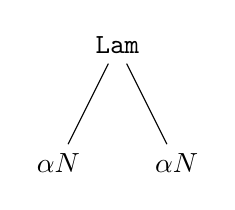
\begin{tikzpicture}
    \begin{scope}[every node/.style={font=\ttfamily}]
    \node (lam) {Lam}
    child {node (var) {$\Binder{\alpha}{\mathbb{N}}$}}
    child {node (var) {$\Var{\alpha}{\mathbb{N}}$}};
    \end{scope}
  \end{tikzpicture}
\end{center}

This syntactic distinction is important because \textsf{Binder}s and \textsf{AST}s need to be distinguished at the type level, and I wish to keep the typing rules syntax directed. To see why it is important to distinguish \textsf{Binder}s and \textsf{AST}s at the \textit{type} level, consider the following malformed AST:
\begin{center}
  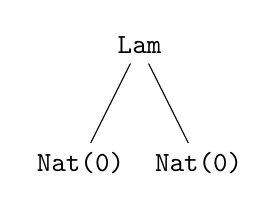
\begin{tikzpicture}
    \begin{scope}[every node/.style={font=\ttfamily}]
    \node (lam) {Lam}
    child {node (var) {Nat(0)}}
    child {node (var) {Nat(0)}};
    \end{scope}
  \end{tikzpicture}
\end{center}

The aforementioned malformed AST should be ill-typed. To do so, it is insufficient to require that the left sub-tree is of type $\textsf{AST($\mathbb{N}$)}$. Thus, \textsf{Binder}s and \textsf{ASTs} should be distinguished at the type level. 

\item \textbf{\texttt{binderToAST}}, a primitive for turning binders (\underline{\texttt{Var}}) into \textit{usages} of binders (\texttt{Var})

This allows us to write programs like the following:
\begin{core}
$\begin{array}{l}
  \textbf{\texttt{do}} \, \, {x} \leftarrow {\Binder{\alpha}{\mathbb{N}}} \, \, \textbf{\texttt{in}} \\
  \textbf{\texttt{do}} \, \, {\texttt{body}} \leftarrow \textbf{\texttt{binderToAST}} \, x \, \, \textbf{\texttt{in}} \\
  \textbf{\texttt{return}} \, \, \texttt{Lam}(x, \texttt{body})
\end{array}$
\vspace{2mm} 
\textcolor{coreComment}{\hrule height 0.2mm \relax}
\vspace{2mm} 

\textcolor{coreComment}{$\begin{array}{l}\return{\texttt{Lam}(\Binder{\alpha}{\mathbb{N}}, \Var{\alpha}{\mathbb{N}})}\end{array}$}
\end{core}

\item $\gensym{T}$, a primitive for generating fresh binders of type $T$ (\underline{\texttt{Var}})

To illustrate why \textbf{\texttt{mkvar}} is necessary, recall that \coreLang{} acts as an elaboration target for \sourceLang{}. Consider the following \sourceLang{} program, which should ideally generate the AST of $\lambda \alpha. \lambda \beta. \, \return{(\alpha, \beta)}$

\begin{source}
$\begin{array}{l}
\$(\textbf{\texttt{do}} \, \, \texttt{mkfun} \leftarrow {\lambda k. \, {\langle\langle\,\, \lambda x: \mathbb{N}^0. \,\, \splice[(k \, {\equote[x]})]\,\, \rangle\rangle}} \, \, \textbf{\texttt{in}} \\
\quad \texttt{mkfun} \,\, (\,\, \lambda a. \, \texttt{mkfun} \, (\lambda b. \, \return{(a, b)})) \,\, )
\end{array}$

\vspace{2mm} 
\textcolor{sourceComment}{\hrule height 0.2mm \relax}
\vspace{2mm} 

\textcolor{sourceComment}{$\begin{array}{l}\return{\texttt{Lam}(\Binder{\alpha}{\mathbb{N}}, \texttt{Lam}(\Binder{\beta}{\mathbb{N}}, \texttt{Ret}(\texttt{Pair}(\Var{\alpha}{\mathbb{N}}, \Var{\beta}{\mathbb{N}}))))}\end{array}$}
\end{source}

The compile-time function \texttt{mkfun} is a higher-order function that takes some compile-time function $k$. $k$ takes in a binder, $x$, and constructs the \textsf{body} of a function $\lambda x. \textsf{body}$. For example, in order to generate the body $x + 1$, we could write 
\[\texttt{mkfun} \,  (\lambda a. \equote[{\splice[(a)]} + 1]) \]
In the example \sourceLang{} program, $k$ calls \texttt{mkfun}. This means that one constructs a \textit{nested} function, whose formal parameters are bound to $a$ and $b$ respectively. If we simply elaborated $x$ into $\Binder{x}{\mathbb{N}}$, we would bind both $a$ and $b$ to $\Binder{x}{\mathbb{N}}$, and generate the following (incorrect) AST: 
 \[\return{\texttt{Lam}(\Binder{x}{\mathbb{N}}, \texttt{Lam}(\Binder{x}{\mathbb{N}}, \texttt{Ret}(\texttt{Pair}(\Var{x}{\mathbb{N}}, \Var{x}{\mathbb{N}}))))}\]
 We thus need to ensure that \texttt{mkfun} is elaborated into a function that generates \textit{fresh} names for $x$ each time it is called. This is the purpose of \textbf{\texttt{mkvar}}. 
\end{enumerate}

Second, I extend \efflang{} with machinery for scope extrusion checking. This comprises:
\begin{enumerate}
\item \err{}, an error state for indicating the presence of scope extrusion,
\item \textbf{\texttt{check}}, a guarded \textbf{\texttt{return}} construct that either detects scope extrusion, and transitions to \textbf{\texttt{err}}, or does not detect scope extrusion, and transitions to \textbf{\texttt{return}},
\item \textbf{\texttt{check$_M$}}, which behaves similarly to \textbf{\texttt{check}}, but (for reasons I will explain in \Cref{section:best-effort-check}) allows a set of \textit{muted} variables $M$ to \textit{temporarily} extrude their scope,
\item \textbf{\texttt{dlet}}, a primitive for tracking which variables are well-scoped and which have extruded their scope,
\item \textbf{\texttt{tls}}, a marker for where top-level splices would have occurred in the source program. This is for \textit{ease of reasoning only}. 
\end{enumerate}

\begin{figure}
\begin{core-desc}
  {\large \textbf{Syntax}} \\

  $\begin{array}{@{}llll}
    \textbf{Normal Forms} & n & ::= & \ldots \mid \Nat{m} \mid \Var{\alpha}{A} \mid \Binder{\alpha}{A} \mid \Lam{n_1}{n_2}  \\ 
  &&&\mid \App{n_1}{n_2} \mid \Continue{n_1}{n_2} \mid \Ret{n}   \\ 
  &&& \mid \Do{n_1}{n_2}{n_3} \mid \Op{n} \mid \Hwith{n_1}{n_2}   \\
  &&&\mid \Hret{n_1}{n_2}(n_1, n_2) \mid \Hop{n_1}{n_2}{n_3}{n_4} \\
  \textbf{Terms} & t & ::= & \ldots \mid \checkfv{n} \mid \checkm{n} \mid \dlet{n}{t} \mid \tls{t} \mid \err \\ &&& \mid \varToAST{n}
  \end{array}$
\end{core-desc}
\caption{\coreLang{} syntax. The syntax is broadly the same as \efflang{}, except with the addition of AST constructors and scope extrusion checking machinery.}
\label{fig:source-syntax}
\end{figure}

Notice that, while the calculus the \textit{machinery} for scope extrusion checking, it does not demand that one \textit{use} it, or use it \textit{properly}. Scope extrusion checking is not a language feature, but an algorithm one builds on top of the calculus. 
\subsection{Operational Semantics}
I will now describe the operational semantics of \coreLang{}. Many rules are identical to those of \efflang{} (\Cref{fig:efflang-opsem}): interesting rules are collated in \Cref{fig:corelang-opsem}. Rules are divided into those related to AST construction (\textsc{Ast-Rule}), and those related to \textbf{s}cope \textbf{e}xtrusion \textbf{c}hecking (\textsc{Sec-Rule}). I will now explain key rules. 

\newcommand{\coreConfiguration}[5]{{#1}; {#2}; {#3}; {#4}; {#5}}
  % \renewcommand{\transition}[2]{#1 & \rightarrow & #2}
  % \renewcommand{\rulename}[2]{(\textsc{{#1}-{#2}})}
  \newcommand{\astRule}[1]{\rulename{Ast}{#1}}
  \newcommand{\secRule}[1]{\rulename{Sec}{#1}}
  % \newcommand{\effectRule}[1]{\rulename{Eff}{#1}}

\begin{figure}[t]
\begin{core-desc}
  \large{\textbf{Operational Semantics}}\\
  \normalsize{\textit{Selected Rules}}\\

  {
    \scriptsize

{\textbf{Evaluation Contexts}}\\
\[F ::= \ldots \mid \dlet{\Binder{\alpha}{A}}{[-]} \mid \tls{[-]} \] 
 {\textbf{Operational Semantics}}\\
\[
  \begin{array}{@{}rrcl}
  \astRule{Sym} & \transition{\coreConfiguration{\gensym{A}}{E}{U}{M}{I}}{\coreConfiguration{\return{\Binder{\alpha}{A}}}{E}{U\cup\{\alpha\}}{M}{I}}\\
  &&&\text{(where $\alpha \notin U$)}\\
  \astRule{Use} & \transition{\coreConfiguration{\varToAST{\Binder{\alpha}{A}}}{E}{U}{M}{I}}{\coreConfiguration{\return{\Var{\alpha}{A}}}{E}{U}{M}{I}}\\
  \vspace{1mm}
  \\ 
  \secRule{Chs} & \transition{\coreConfiguration{\checkfv{n}}{E}{U}{M}{I}}{\coreConfiguration{\return{n}}{E}{U}{M}{I}}\\
    &&&\text{(if $\freevars{n} \subseteq \projfvs{E}$)}\\
  \secRule{Chf} & \transition{\coreConfiguration{\checkfv{n}}{E}{U}{M}{I}}{\coreConfiguration{\err}{E}{U}{M}{I}}\\
  &&&\text{(if $\freevars{n} \not\subseteq \projfvs{E}$)}       \\\vspace{1mm}\\
  \secRule{Cms} & \transition{\coreConfiguration{\checkm{n}}{E}{U}{M}{I}}{\coreConfiguration{\return{n}}{E}{U}{M}{I}}\\
    &&&\text{(if $\freevars{n} \setminus M \subseteq \projfvs{E}$)}\\
  \secRule{Cmf} & \transition{\coreConfiguration{\checkm{n}}{E}{U}{M}{I}}{\coreConfiguration{\err}{E}{U}{M}{I}}\\
  &&&\text{(if $\freevars{n} \setminus M \not\subseteq \projfvs{E}$)}
\\ 
 \vspace{1mm}
\\
\secRule{Tls} & \transition{\coreConfiguration{\tls{\return{n}}}{E}{U}{M}{I}}{\coreConfiguration{\return{n}}{E}{U}{M'}{I'}}\\\vspace{1mm}
\\
  \secRule{Dlt} & \transition{\coreConfiguration{\dlet{\Binder{\alpha}{T}}{\return{n}}}{E}{U}{M}{I}}{\coreConfiguration{\return{n}}{E}{U}{\textcolor{coreHighlight}{M'}}{\textcolor{coreHighlight}{I'}}}\\
   &&&\text{\textcolor{coreHighlight}{(if $ I < \textsf{len}(E)$ then $M' = M, I' = I$}}\\
   &&&\text{\textcolor{coreHighlight}{else $M' = \emptyset, I' = \top$)}}\\
   \effectRule{Op} & \transition{\coreConfiguration{\op{v}}{E_1[\handleWith{E_2}{h}]}{U}{M}{I}}\coreConfiguration{c[v/x, \text{cont}/ k]}{E_1}{U}{\textcolor{coreHighlight}{M \cup \projfvs{E_2}}}{\textcolor{coreHighlight}{I'}}\\
  &&& \text{(where cont $=\kappa x. \, \handleWith{E_2[\return{x}]}{h}$}\\
  &&& \text{and $\opHandler{x}{k}{c} \in h$ and $\textbf{\textsf{op}} \notin \textsf{handled}(E_2)$}\\
  &&& \text{and \textcolor{coreHighlight}{$I' = \textsf{min}(\textsf{len}(E), I)$)}}
  \end{array} \]
  }
\end{core-desc}
\caption{Selected rules of the \coreLang{} operational semantics. Many of the rules can be trivially adapted from the \efflang{} semantics (\Cref{fig:efflang-opsem}). The muting and unmuting of variables is complex, and will be best explained when we discuss scope extrusion checks. For now, these mechanisms are \textbf{\textcolor{coreHighlight}{highlighted}}.}%
\label{fig:corelang-opsem}
\end{figure}

\subsubsection{Configurations}
Like \efflang{}, the operational semantics is defined over \textit{configurations}. In \coreLang{}, configurations have the form:
\[\langle t; E; U; M; I \rangle\]
I will describe each element of the configuration at a high level: their roles will become clearer as we introduce each rule. $t$ and $E$ are as they are in \efflang{}: terms and evaluation contexts. $U$ acts as a source of freshness for name generation. $M$ is a set of muted variables, i.e. those that we do not want to trigger a scope extrusion error, even if they have extruded their scope. $I$ indicates the point at which we should \textit{unmute}, setting $M$ to $\emptyset$. 

\subsubsection{AST Rules}
The \textsc{Ast-Gen} rule describes the behaviour of \textbf{\texttt{mkvar}}: $\gensym{T}$ produces a \texttt{Var} of type $T$ and some name $\alpha$. Recall that names should be \textbf{fresh}: that is, multiple calls to \textbf{\texttt{mkvar}} should always return variables with different names. In order to ensure that names are fresh, we need to keep track of names that have been previously generated. This is the purpose of $U$ in the configuration, and the side condition on the rule. To ensure determinacy of the semantics, we will assume that names are chosen \textit{deterministically}.

The other primitive, \textbf{\texttt{binderToAST}}, turns binders $\Binder{\alpha}{T}$ into usages of the binder $\Var{\alpha}{T}$ (\textsc{Ast-Use}). 

\subsubsection{Scope Extrusion Checking Rules}
More interesting are the primitives for scope extrusion checking. The \textbf{\texttt{check}} primitive acts like a guarded \textbf{\texttt{return}}, which can catch occurrences of scope extrusion. For some arbitrary $n$ of AST type, either:
\begin{enumerate}
  \item All the free variables of $n$ are properly scoped, so $\checkfv{n}$ reduces to $\return{n}$ (\textsc{Sec-Chs})
  \item Some free variables of $n$ are not properly scoped, so $\checkfv{n}$ reduces to $\err$ (\textsc{Sec-Chf})
\end{enumerate}
What does it mean to be ``properly scoped'' (the side condition on \textsc{Sec-Chs})? The answer is slightly subtle. Consider the following program 
\[\bind{\texttt{body}}{\checkfv{n}}{\checkfv{\Lam{\Var{\alpha}{\mathbb{N}}}{\texttt{body}}}}\]
I argue that $\Var{\alpha}{\mathbb{N}}$ \textbf{ought to be} properly scoped in $n$ (should not cause a transition to $\err$). However, it is hard to deduce this from the \textit{static} structure of the program. Instead, one has to reason about the \textit{dynamic} execution of the program. Rather than calculating what is properly scoped as a \textit{language feature}, I defer it to the programmer. The programmer must \textit{declare} that a variable is properly scoped through use of the \textbf{\texttt{dlet}} keyword. 
\[\dlet{\Binder{\alpha}{\mathbb{N}}}{\bind{\texttt{body}}{\checkfv{n}}{\checkfv{\Lam{\Var{\alpha}{\mathbb{N}}}{\texttt{body}}}}}\]
More precisely, \textbf{\texttt{dlet}} places a frame of the form $\dlet{\Binder{\alpha}{A}}{[-]}$ on the evaluation context $E$. I use the notation $\projfvs{E}$ to filter out variables declared in this manner. For example,
\[\projfvs{\dlet{\Binder{\alpha}{A}}{\bind{x}{[-]}{t}}} = \{ \Var{\alpha}{A} \}\]

Given a term of the form $\checkfv{n}$ in some evaluation context $E$, where $n$ is an AST, \textbf{\texttt{check}} thus checks that the free \texttt{Var}s of $n$, written $\freevars{n}$, have all been properly declared, or to be precise, a subset of $\projfvs{E}$. 

It may seem lazy of me to define the semantics of \textbf{\texttt{check}} in such a way that places the burden onto the user. Recall, however, that \coreLang{} is \textit{not} meant to be programmed in directly. Rather, it acts as an elaboration target for \sourceLang{}, and I define the elaboration. Therefore, I am the (only) \coreLang{} user, and the onus is on me to justify that my elaboration uses \textbf{\texttt{check}} appropriately. 

I also introduce \textbf{\texttt{check}}$_M$ as a variant of \textbf{\texttt{check}}. As I will explain in \Cref{section:best-effort-check}, to design a good scope extrusion check, it is necessary to \textit{mute} some variables, pretending that they are properly scoped. \textbf{\texttt{check}}$_M$ will behave exactly like \textbf{\texttt{check}}, except that it will also pretend the muted variables $M$ are properly scoped.

Similarly, when justifying the correctness of scope extrusion checks, it will be useful to remember the position of top-level splices in the \sourceLang{} source program. This is the purpose of \textbf{\texttt{tls}}, which should be interpreted as a no-op (\textsc{Sec-Tls}).

The final two rules, \textsc{Sec-Dlt} and \textsc{Eff-Op}, behave as normal, but additionally mute or unmute \texttt{Var}s. The operations of muting and unmuting are best explained in [THE NEXT CHAPER]. For now, they are \textbf{\textcolor{coreHighlight}{highlighted}}, and can be mostly ignored. At a high level, when an operation is performed, we mute some set of variables, and potentially update the point at which they should be unmuted. When we remove a declared variable, we additionally check if we ought to unmute variables (and do so if we should).

\subsection{Type System}
Extending the types is similarly straightforward. I add only two types: a \textsf{Binder} type and an \textsf{AST} type. The types are summarised in \Cref{fig:core-types}.

\begin{figure}[t]
  \begin{core-desc}
    {\large {\textbf{Types}}}\\
    \textit{Computation and Handler Types omitted}\\

    \textbf{Run-time Pre-types}\\
    $\begin{array}{@{}lllr}
    \text{Effects Row} & \xi ::= \emptyset \mid \xi \cup \{ \texttt{op}_i \} \\
    \\
    \text{Value type} & A ::= \mathbb{N} & \\
                              &\quad\quad\,\,\, \mid \functionType[\xi]{A_1}{A_2} & \text{functions}\\
                              &\quad\quad\,\,\, \mid \continuationType[\xi]{A_1}{A_2} & \text{continuations}\\ \\
    \text{Computation type} & \effectType[\xi]{A} \\
    \text{Handler type} & \handlerType{\effectType[\xi]{A_1}}{\effectType[\xi']{A_2}}
    \end{array}$
    
    \vspace{4mm}

    \textbf{Types}\\
  $\begin{array}{@{}lllr}
    % \text{Effects Row} & \Delta ::= \emptyset \mid \Delta \cup \{ \texttt{op}_i \} \\
    % \\
    % \text{}
    \text{Value type} & T ::= \ldots\\
                              &\quad\quad\,\,\, \mid \textsf{Binder}(A) & \text{binders}\\
                              &\quad\quad\,\,\, \mid \textsf{AST}(A) & \text{AST (value)}\\
                              &\quad\quad\,\,\, \mid \textsf{AST}(\effectType[\xi]{A}) & \text{AST (computation)}\\
                              &\quad\quad\,\,\, \mid \textsf{AST}(\handlerType{\effectType[\xi]{A_1}}{\effectType[\xi']{A_2}}) & \text{AST (handler)}\\
    % \text{Computation type} & \effectType{T} \\
    % \text{Handler type} & \handlerType{\effectType{T_1}}{\effectType[\Delta']{T_2}}
  \end{array}$
  \end{core-desc}
  \caption{The types of \coreLang{}. \coreLang{} types extend \efflang{} types with an \textsf{AST} type (for ASTs), and a \textsf{Binder} type}%
  \label{fig:core-types}
\end{figure}

% The role of the \textsf{AST} type is clear, but the role of \textsf{Binder} less so. I illustrate the purpose of the \textsf{Binder} type by example. Consider the following malformed AST:

% \begin{center}
%   \begin{tikzpicture}
%     \begin{scope}[every node/.style={font=\ttfamily}]
%     \node (lam) {Lam}
%     child {node (var) {Nat($0$)}}
%     child {node (var) {Nat($0$)}};
%     \end{scope}
%   \end{tikzpicture}
% \end{center}

% The aforementioned malformed AST should be ill-typed. To do so, it is insufficient to require that the left sub-tree is of type $\textsf{AST($\mathbb{N}$)}$. It must specifically be a \underline{\textsf{Var}} AST node. That is the purpose of the \textsf{Binder} type. 

\subsubsection{Typing Rules}
I now describe a selection of \coreLang{} typing rules (\Cref{fig:core-typing-rules}). The rules are extremely straightforward: $\Binder{\alpha}{A}$ is a \textsf{Binder} of type $A$, and $\Var{\alpha}{A}$ is an \textsf{AST} of type $A$. $\gensym{A}$ is a computation that produces \textsf{Binder}s of type $A$, and $\Lam{n_1}{n_2}$ is well-typed if $n_1$ is a \textsf{Binder} and $n_2$ an AST. 

Notice that this type system does not guarantee that the resulting AST is \textit{well-scoped}, for example, the following is well-typed:
\[\cdot \vdash {\Var{\alpha}{A}}: {\textsf{AST}(A)}\]

The typing rules for scope extrusion checks are even more straightforward: they are effectively invisible to the type system. The only complex case is \textbf{\texttt{err}}, which can be assigned any type in any context. \textbf{\texttt{err}} thus behaves similarly to \textbf{\texttt{absurd}} in \texttt{Haskell}, or in the $\lambda$-calculus extended with the empty type \citep{scherer-2017}.

Finally, I define the notion of well-typed term. 
\begin{definition}[Well-typed term]{coreHighlight}
A term $t$ is well-typed if $\cdot \vdash t: T \, ! \,  \emptyset$
\end{definition}
\begin{figure}
  \begin{core-desc}
    {\large \textbf{Typing Rules}}\\
    \textit{Selected Rules}
    \begin{center} 
    \begin{minipage}[t]{0.32\textwidth}
      \centering
    $\inferrule[(Binder)]{  }{\type{\Binder{\alpha}{A}}{\textsf{Binder}(A)}}$
    \end{minipage}%
    \begin{minipage}[t]{0.32\textwidth}
      \centering
    $\inferrule[(Variable)]{  }{\type{\Var{\alpha}{A}}{\textsf{AST}(A)}}$
    \end{minipage}%
    \begin{minipage}[t]{0.36\textwidth}
      \centering
    $\inferrule[(Mkvar)]{  }{\type{\gensym{A}}{\effectType{\textsf{Binder}(A)}}}$
    \end{minipage}

      \vspace{5mm}

      \begin{minipage}[t]{0.4\textwidth}
      \centering
     $\inferrule[(BinderToAST)]{\type{n}{\textsf{Binder}(A)}}{\type{\varToAST{n}}{\effectType{\textsf{AST}(A)}}}$
    \end{minipage}%
    \begin{minipage}[t]{0.6\textwidth}
      \centering
    $\inferrule[(Lambda-AST)]{\type{n_1}{\textsf{Binder}(A_1)}\\{\type{n_2}{\textsf{AST}(\effectType[\xi]{A_2})}}}{\type{\Lam{n_1}{n_2}}{\textsf{AST}(\functionType[\xi]{A_1}{A_2})}}$
    \end{minipage}

    \vspace{5mm}

    \begin{minipage}[t]{0.25\textwidth}
      \centering
    $\inferrule[(Err)]{    }{\type{\err}{\effectType{T}}}$
    \end{minipage}%
    \begin{minipage}[t]{0.25\textwidth}
      \centering
    $\inferrule[(Tls)]{\type{t}{\effectType{T}}}{\type{\tls{t}}{\effectType{T}}}$
    \end{minipage}%
    \begin{minipage}[t]{0.5\textwidth}
      \centering
    $\inferrule[(DLet)]{\type{n}{\textsf{Binder}(A)} \\ \type{t}{\effectType{T}}}{\type{\dlet{n}{t}}{\effectType{T}}}$
    \end{minipage}

    % \vspace{5mm}

    % \begin{minipage}[t]{\textwidth}
    %   \centering
    % $\inferrule[(BinderToAST)]{\type{n}{\textsf{Binder}(A)}}{\type{\varToAST{n}}{\textsf{AST}(A)}}$
    % \end{minipage}

    \vspace{5mm}

    \begin{minipage}[t]{\textwidth}
      \centering
    $\inferrule[(Check)]{\type{n}{T} \\ T = \textsf{AST}(A) \lor \textsf{AST}(\effectType[\xi]{A}) \lor \textsf{AST}(\handlerType{\effectType[\xi]{A_1}}{\effectType[\xi']{A_2}})}{\type{\checkfv{n}}{\effectType{T}}}$
    \end{minipage}

  \end{center}
  \end{core-desc}

\caption{Selected \coreLang{} typing rules}
\label{fig:core-typing-rules}
\end{figure}
 
\subsection{Implementation}
The core calculus \coreLang{} describes abstractly a concrete \texttt{OCaml} implementation. In the concrete \texttt{OCaml} implementation, we do not need to introduce \textbf{\texttt{check}}, \textbf{\texttt{dlet}}, and \textbf{\texttt{err}} as primitives. Rather, they can be encoded as a \textit{mode of use} of effects and handlers. 
\begin{enumerate}
  \item $\checkfv{n}$ is implemented by performing a \texttt{FreeVar} effect, that are passed the free variables of $n$\\ 
  $\checkm{n}$ is similar, except there are also \texttt{Mute} and \texttt{Unmute} effects
  
  \item $\dlet{\Binder{\alpha}{T}}{t}$ is implemented as a \textit{handler} of the \texttt{FreeVar} effect, which subtracts $\Var{\alpha}{T}$ from the set of free variables, and either:
  \begin{enumerate}
    \item Resumes the continuation, if the set of free variables is now empty (all free variables properly declared/scoped)
    \item Performs another \texttt{FreeVar} effect, to check that the remaining free variables are properly declared. Following a successful such check, the continuation may be resumed.
  \end{enumerate}
  \item \textbf{\texttt{err}} is an unhandled \texttt{FreeVar} effect
\end{enumerate}

\section{Elaboration from \texorpdfstring{\sourceLang{}}{Lambda-Op-Quote-Splice} to \texorpdfstring{\coreLang{}}{Lambda-Op-AST}}\label{section:elaboration}
Having described both \sourceLang{} and \coreLang{}, I will now describe a simple elaboration from \sourceLang{} to \coreLang{}. This elaboration will be \textit{simple} -- it will not insert any dynamic scope extrusion checks.

\newcommand{\elaborate}[1]{\llbracket #1 \rrbracket}
\newcommand{\erase}[1]{\textsf{erase}(#1)}
\newcommand{\AST}[1]{\textsf{AST}(#1)}
\newcommand{\Code}[1]{\textsf{Code}(#1)}


The elaboration is defined on typing judgements: I elaborate a \sourceLang{} judgement to a \coreLang{} judgement. To do so, I define four elaborations: on effect rows, types, contexts, and terms. As it will be clear from context which elaboration is being referred to, I will abuse notation and write $\llbracket - \rrbracket$ for all four.

Elaborating effect rows will just be the identity, that is 
\[\begin{array}{rcl}
  \elaborate{\Delta} &=& \Delta \\
  \elaborate{\xi}&=&{\xi}
\end{array}\]
and I will not touch on them any further. 

\subsection{Elaborating Types}
To define elaboration of types, it will be convenient to refer to a helper function, \textsf{erase}, that \textit{erases} all of the level annotations (and elaborates effect rows). It is easy to define inductively, and I do not give a formal definition, but rather an example. 
\[\textsf{erase}((\functionType[\xi]{T_1^0}{T_2^0})^0) = \functionType[\elaborate{\xi}]{T_1}{T_2}\]
I can now define elaboration of types easily. In a nutshell, level $0$ types elaborate into \textsf{AST} types. Level $-1$ types elaborate into themselves (sans level annotations), except for \textsf{Code} types, which elaborate into \textsf{AST} types.
\[
\begin{array}{rcl}
  \elaborate{T^0} & = & \AST{\erase{T^0}}\\
  \elaborate{\effectType[\xi]{T^0}} & = & \AST{\erase{\effectType[\xi]{T^0}}}\\
  \elaborate{\effectType[\Delta]{T^0}} & = & \effectType[\elaborate{\Delta}]{\AST{\erase{T^0}}}\\
  \elaborate{\effectType[\Delta ; \xi]{T^0}} & = & \effectType[\elaborate{\Delta}]{\AST{\erase{\effectType[\xi]{T^0}}}}\\
  \elaborate{{(\handlerType{\effectType[\xi]{T_1^0}}{\effectType[\xi']{T_2^0}})}^0} & = & {\AST{\erase{(\handlerType{\effectType[\xi]{T_1^0}}{\effectType[\xi']{T_2^0}})^0}}}\\\\
  \elaborate{T^{-1}} & = & \text{if} \, T \neq \Code{\effectType[\xi]{T^0}} \, \text{then} \, \erase{T^{-1}} \\ && \text{else}\, \AST{\erase{\effectType[\xi]{T^0}}}\\
  \elaborate{\effectType{T^{-1}}} & = & \effectType[\elaborate{\Delta}]{\elaborate{T^{-1}}}\\
  \elaborate{{(\handlerType{\effectType[\Delta]{T_1^{-1}}}{\effectType[\xi']{T_2^{-1}}})}^{-1}} & = & {\AST{\erase{(\handlerType{\effectType[\Delta]{T_1^{-1}}}{\effectType[\xi']{T_2^{-1}}})^{-1}}}}
\end{array}
\]
\subsection{Elaborating Contexts}
Elaborating contexts is \textit{slightly} subtle. Rather than mapping the elaboration function over all types in the context, we treat the level $0$ types slightly differently, elaborating in \textsf{Binder}, rather than \textsf{AST} types. 
\[
\begin{array}{rcl}
  \elaborate{\cdot} & = & \cdot \\
  \elaborate{\Gamma, x:T^0} & = & \elaborate{\Gamma}, x: \textsf{Binder}(\erase{T^0})\\
  \elaborate{\Gamma, x:T^{-1}} & = & \elaborate{\Gamma}, x: \elaborate{T^{-1}}
\end{array}
\]
To see why this is the case, notice that the only cases where the context $\Gamma$ is extended with a level $0$ variable $x: T^0$ occur in \compilemode{} or \quotemode{}. In these modes, we are building ASTs, and thus $x$ must be an AST \textsf{Binder}. 
% \subsection{Elaborating Effects}

\subsection{Elaborating Terms}
Elaborating terms is slightly more involved. To start, we will assume that we have annotated all binders with their types, for example 
\[\lambda x: \mathbb{N}^0. \, e\]
The elaboration for terms is moderated by the \textbf{mode}: \compilemode{}, \quotemode{}, or \splicemode{}. Selected rules are collated in \Cref{fig:term-elaboration}. 

At a high level, in \compilemode{} and \quotemode{}-mode, one builds ASTs, calling \textbf{\texttt{mkvar}} when binders are encountered (see earlier discussion on the necessity of \textbf{\texttt{mkvar}}). Elaboration in \compilemode{} and \quotemode{}-modes do not differ particularly significantly, with the exception of the rule for splice, where in \compilemode{}, I insert the marker for the top-level splice, and in \quotemode{}, I do not. Elaboration in \compilemode{} and \quotemode{}-modes will be further distinguished when I extend the elaboration to insert scope extrusion checks. Elaboration in \splicemode{}-mode is effectively the identity. 

\newcommand{\cqmode}{\compilemode{} \mid \quotemode{}}
\begin{figure}
  \begin{source-desc}
    {\large\textbf{Term Elaboration}}\\
    \textit{Selected Rules}

    {\footnotesize
    \[
    \begin{array}{@{}lll}
      \elaborate{x}_{\cqmode} & = & \varToAST{x}\\
      \elaborate{\lambda x: T^0. \, e}_{\cqmode} & = & \bind{x}{\gensym{\erase{T^0}}}{\bind{\texttt{body}}{\elaborate{e}_{\cqmode}}{\return{\Lam{x}{\texttt{body}}}}}\\\\
      \elaborate{\splice}_{\compilemode{}} & = & \tls{\elaborate{e}_{\splicemode{}}}\\
      \elaborate{\splice}_{\quotemode{}} & = & {\elaborate{e}_{\splicemode{}}}
      \\\\
      \elaborate{x}_{\splicemode{}} & = & x\\
      \elaborate{\lambda x: T^0. \, e}_{\splicemode{}} & = & \lambda x. \elaborate{e}_{\splicemode{}}\\
      \elaborate{\equote}_{\splicemode{}} & = & \elaborate{e}_{\quotemode{}}
    \end{array}
    \]
    }
  \end{source-desc}
  \caption{Selected term elaboration rules from \sourceLang{} to \coreLang{}. Elaboration is moderated by the compiler mode. In \compilemode{} and \quotemode{}, elaboration builds ASTs. In \splicemode{}-mode, elaboration is effectively the identity. }%
  \label{fig:term-elaboration}
\end{figure}

\subsection{Elaborating Typing Judgements}
We may now elaborate full typing judgements, by elaborating each component in the judgement. For example, take the typing judgement for lambdas in \compilemode{}-mode. 
\[
{\inferrule{\ctypejudge[\Gamma, x: T_1^0]{e}{\runtimecomptype{T_2}{\Delta;\xi}}}{\ctypejudge{\lambda x.e}{\runtimecomptype{(\functionType[\xi]{T_1^0}{T_2^0})}{\Delta}}}}
\]
which we elaborate by applying the elaboration component-wise
\newcommand{\typejudge}[3][\Gamma]{#1 \vdash #2 : #3}
\[
{\inferrule{\typejudge[\elaborate{\Gamma, x: T_1^0}]{\elaborate{e}_{\compilemode{}}}{\elaborate{\runtimecomptype{T_2}{\Delta;\xi}}}}{\typejudge[\elaborate{\Gamma}]{\elaborate{\lambda x.e}_{\compilemode{}}}{\elaborate{\runtimecomptype{(\functionType[\xi]{T_1^0}{T_2^0})}{\Delta}}}}}
\]
Letting $A_i = \erase{T_i^0}$, and $\elaborate{e}_{\compilemode{}} = t$, and applying the elaboration functions defined above, we obtain
{
\[
{\inferrule{\typejudge[\elaborate{\Gamma}, x: \textsf{Binder}(A_1)]{t}{\effectType{\AST{\effectType[\xi]{A_2}}}}}{\typejudge[\elaborate{\Gamma}]{\bind{x}{\gensym{\erase{T^0}}}{\bind{\texttt{body}}{t}{\return{\Lam{x}{\texttt{body}}}}}}{\effectType{\AST{\functionType[\xi]{A_1}{A_2}}}}}}
\]
}
which, assuming that the premise is valid typing derivation, corresponds to a valid \sourceLang{} typing derivation.

Is this true in general? Do \sourceLang{} typing derivations always elaborate into \coreLang{} typing derivations? Yes, but the question begets a larger point: what properties can we claim about the calculus as defined? What metatheoretic results may we establish?
\section{Metatheory}\label{section:metatheory}
I now establish several metatheoretic properties of the \sourceLang{} calculus.

The first states that well-typed \sourceLang{} programs elaborate into well-typed \coreLang{} programs.

\begin{theorem}[Elaboration Preservation]{sourceHighlight}
  If $\Gamma \vdash_{\star} e: \tau$ then $\elaborate{\Gamma} \vdash \elaborate{e}_{\star}: \elaborate{\tau}$, where $\star = \compilemode{} \mid \quotemode{} \mid \splicemode{}$ and $\tau$ is a level $0$ or level $-1$ value, computation, or handler type. 
\end{theorem}

The proof is by induction on the typing rules, as in the example in the previous section.  

We can also prove that the core language \coreLang{} satisfies appropriate progress and preservation properties. 

\begin{theorem}[Progress]{coreHighlight} 
If $\type{E[t]}{\effectType{T}}$ then for all $U, M, I$ either 
\begin{enumerate}
\item $t$ of the form $\return{n}$ and $E = [-]$,
\item $t$ of the form $\op{v}$ for some $\textsf{op} \in \Delta$,
\item $t$ of the form $\err$
\item $\exists t', E', U', M', I'$ such that $\langle t; E; U; M; I \rangle \rightarrow \langle t';E';U';M';I'\rangle$
\end{enumerate}
\end{theorem}
Note that I additionally have to consider the error state \textbf{\texttt{err}}. Progress is proved by induction over the typing derivation. Since I am extending \efflang{}, I only need to consider the augmented typing rules, all of which are extremely straightforward.

\begin{theorem}[Reduction Preservation]{coreHighlight}
If 
\begin{enumerate} 
  \item $\Gamma \vdash E[t]: T$ and 
  \item $\langle t; E; U; M; I \rangle \to \langle t'; E'; U'; M'; I' \rangle$ 
  \end{enumerate}
  then $\Gamma \vdash E'[t']: T$ 
\end{theorem}
Proof proceeds by induction over the operational semantics. Once again, I only need to consider the augmented rules, which are very simple. 

As a corollary, we get a notion of type safety.
\begin{corollary}[Type Safety]{sourceHighlight}\label{cor:core-type-safety}
  If $\ctypejudge[\cdot]{e}{T^0 \, ! \, \emptyset;\emptyset}$ then either
  \begin{enumerate}
    \item $\langle \elaborate{e}_{\compilemode{}}; [-]; \emptyset
    ; \emptyset; \top \rangle \to^{\omega}$,
    \item $\langle \elaborate{e}_{\compilemode{}}; [-]; \emptyset; \emptyset; \top \rangle \to^{*} \langle \err; E; U; M; I \rangle$ for some $E$, $U$, $M$, $I$, or 
    \item $\langle \elaborate{e}_{\compilemode{}}; [-]; \emptyset; \emptyset; \top \rangle \to^{*} \langle \return{n}; [-]; U; M; I \rangle$ for some $U$, $M$, $I$
  \end{enumerate} 
\end{corollary}

Importantly, this notion of type safety is weak. A system which always reports a scope extrusion error (\textbf{\texttt{err}}) would be type safe. Further, a system which never reports scope extrusion would be type safe as well. Due to the potential presence of scope extrusion, in the third case of \Cref{cor:core-type-safety}, we cannot additionally claim that the normal form $n$ represents a well-typed \efflang{} program. 

% In addition to type safety, we can formulate an equational theory for \sourceLang{}. First, I prove that, underneath a top-level splice, splice and quotation are duals. Second, I prove that \sourceLang{} is a fine-grain CBV calculus. 

% To formulate this equational theory, we will need a notion of contextual equivalence in \coreLang{}. In turn, this demands a notion of equality between \textsf{AST}s of values, computations, and handlers. I will abuse notation and write $n_1 =_\textsf{AST} n_2$, to represent all three. The notion of equality I choose is syntactic equality up to $\alpha$-renaming. So, for example, 
% \renewcommand{\Var}[2]{\texttt{Var}(#1_{#2})}

% \begin{center}
% \begin{tikzpicture}
%       \node (equals) {$=_{\textsf{AST}}$};

%   \begin{scope}[every node/.style={font=\ttfamily}, shift={($(equals.west) + (-3cm, 0.7cm)$)}]
%     \node (lam) {Lam}
%     child {node (var) {$\Binder{\alpha}{\mathbb{N}}$}}
%     child {node (var) {$\Var{\alpha}{\mathbb{N}}$}};
%     \end{scope}


%   \begin{scope}[every node/.style={font=\ttfamily}, shift={($(equals.east) + (3cm, 0.7cm)$)}]
%     \node (lam) {Lam}
%     child {node (var) {$\Binder{\beta}{\mathbb{N}}$}}
%     child {node (var) {$\Var{\beta}{\mathbb{N}}$}};
%     \end{scope}
    
% \end{tikzpicture}
% \end{center}
% but, however, 
% \begin{center}
% \begin{tikzpicture}
%       \node (equals) {$\neq_{\textsf{AST}}$};

%   \begin{scope}[every node/.style={font=\ttfamily}, shift={($(equals.west) + (-3cm, 0.7cm)$)}]
%     \node (lam) {Plus}
%     child {node (var) {1}}
%     child {node (var) {2}};
%     \end{scope}


%   \begin{scope}[every node/.style={font=\ttfamily}, shift={($(equals.east) + (3cm, 0.7cm)$)}]
%     \node (lam) {Plus}
%     child {node (var) {2}}
%     child {node (var) {1}};
%     \end{scope}
    
% \end{tikzpicture}
% \end{center}
% Syntactic equality is, of course, not the only sensible notion of equality. One can also choose, for example, contextual equivalence with respect to the \efflang{} semantics. Nevertheless, armed with this notion of equality on \textsf{AST} types, it is easy to define a notion of contextual equivalence in \coreLang{}. First, define ground types 
% \[T_\textsf{Ground} \triangleq \mathbb{N} \mid \textsf{AST}(A) \mid \textsf{AST}(\effectType[\xi]{A}) \mid \textsf{AST}(\handlerType{\effectType[\xi]{A_1}}{\effectType[\xi']{A_2}})\]
% and a notion of equality on each ground type ($=_{\textsf{Ground}}$), which is just numerical equality for $\mathbb{N}$ and $=_{\textsf{AST}}$ for AST types. Then,
% \begin{definition}[Contextual Equivalence]{coreHighlight}\label{dfn:ctx-equiv}
%   $t$ and $t'$ are contextually equivalent at context $\Gamma$ and type $\effectType{T}$, written $\Gamma \vdash t \contextequiv t': '\effectType{T}$ if 
%   \begin{enumerate}
%     \item $\type{c}{\effectType{T}}$ and $\type{c'}{\effectType{T}}$
%     \item For all $E$ such that $\cdot \vdash {E[c]}: {\effectType[\emptyset]{T_{\textsf{Ground}}}}$  and $\cdot \vdash {E[c']}: {\effectType[\emptyset]{T_{\textsf{Ground}}}}$, we have either 
%     \begin{enumerate}
%       \item $\langle t; E; []; \emptyset; \top \rangle \to^{\omega}$ and $\langle t'; E; []; \emptyset; \top \rangle \, \to^{\omega}$,
%       \item For some $E_1$, $M_1$, $U_1$, $I_1$, $E_2$, $M_2$, $U_2$, $I_2$\\ $\langle t; E; []; \emptyset; \top \rangle \to^{*} \langle \err; E_1; M_1; U_1; I_1 \rangle$, and \\
%       $\langle t'; E; []; \emptyset; \top \rangle \to^{*} \langle \err; E_2; M_2; U_2; I_2 \rangle$
%       \item For some $M_1$, $U_1$, $I_1$, $M_2$, $U_2$, $I_2$\\ $\langle t; E; []; \emptyset; \top \rangle \to^{*} \langle \return{n}; [-]; M_1; U_1; I_1 \rangle$, and \\
%       $\langle t'; E; []; \emptyset; \top \rangle \to^{*} \langle \return{m}; [-]; M_2; U_2; I_2 \rangle$, and \\ 
%       $n =_{\textsf{Ground}} m$ 
%     \end{enumerate}
%     %  \, {\effconfiguration{\return{v}}{[-]}} \iff \effconfiguration{c'}{E} \, \to^{*} \, \effconfiguration{\return{v}}{[-]}
%   \end{enumerate}
% \end{definition}

% We can now prove the equational theory of \sourceLang{}. 

Additionally, underneath a top-level splice, splice and quotation are duals. That is, 
\begin{theorem}[Quote-Splice Duality]{sourceHighlight}
\[\begin{array}{rcl}
\splice[{\equote}] & =_{\quotemode{}} & e \\
\equote[{\splice}] & =_{\splicemode{}} & e
\end{array}
\]
\end{theorem}
Where, in this context, $=_{\star}$ means ``elaborates to contextually equivalent \coreLang{} programs in $\star$ mode''. Parameterising by the mode is necessary, since the mode will affect the result of elaboration. Indeed, we may prove something stronger: they elaborate to the same \coreLang{} program (contextual equivalence follows from reflexivity). Proof is by inspection of the definition of elaboration, where
\[\begin{array}{rcl}  
  \elaborate{\splice[{\equote}]}_{\quotemode{}} = t & \iff & \elaborate{e}_{\quotemode{}} = t\\
  \elaborate{\equote[{\splice}]}_{\splicemode{}} = t & \iff & \elaborate{e}_{\splicemode{}} = t
\end{array}
  \]

% To prove that \sourceLang{} is a fine-grain CBV calculus (\Cref{dfn:fine-grain-cbv}) is only slightly more involved.  

% [TODO]